% chktex-file 44

\chapter{Methods}
\label{ch:methods}
This chapter presents the methodology of the proposed hybrid semantic exploration system, 
designed to mitigate the key limitations identified in Chapter~\ref{ch:sota}, namely the 
absence of persistent semantic memory, the reliance on single-source semantic detections, 
and the lack of an explicit and controllable trade-off between semantic exploration and 
exploitation in existing approaches.

The proposed system integrates zero-shot semantic perception with frontier-based exploration and persistent 3D semantic mapping into a unified, closed-loop decision-making framework. Semantic evidence acquired during exploration is continuously fused into a long-term spatial memory, while exploration behavior is adaptively modulated based on the reliability of accumulated semantic beliefs.

An overview of the system architecture is provided in Section~\ref{sec:methods:system_overview}, followed by detailed descriptions of the core components: semantic frontier exploration (Section~\ref{sec:methods:semantic_frontier}), promptable zero-shot detection (Section~\ref{sec:methods:zero_shot_detection}), persistent semantic 3D mapping (Section~\ref{sec:methods:persistent_mapping}), the multi-source fusion strategy governing semantic belief updates (Section~\ref{sec:methods:fusion_strategy}), and the behavior tree used to orchestrate semantic-guided exploration and navigation (Section~\ref{sec:methods:behavior_tree}).


\section{System Overview}
\label{sec:methods:system_overview}

The proposed system follows a modular hybrid architecture that tightly couples semantic perception,
geometry-driven exploration, and persistent semantic mapping to enable robust open-vocabulary
object-guided exploration. Figure~\ref{fig:system_overview} provides a high-level overview of the system components and their data flow. The exploration task is specified by a user-provided natural language prompt, which defines the semantic target and conditions the detection, exploration, and fusion modules throughout system execution.

\begin{figure}[h!]
    \centering
    \includegraphics[width=\textwidth]{Images/03_methods/sage_pipeline.png}
    \caption{Overview of the SAGE system architecture for open-vocabulary semantic exploration.
    RGB-D observations and robot poses are processed by three parallel modules: 
    (a) a persistent semantic mapping backend (OpenFusion~\cite{yamazakiOpenFusionRealtimeOpenVocabulary2023}) that maintains a semantic 3D map, 
    (b) a semantic frontier exploration module that scores geometric frontiers based on language-guided relevance, and 
    (c) a promptable zero-shot detection pipeline for object hypotheses.
    All semantic hypotheses are represented as graph nodes, filtered by relevance maps, and fused using a multi-source fusion strategy.
    A behavior tree orchestrates exploration, verification, and navigation actions, while low-level motion planning and execution are handled by the ROS~2 Navigation Stack~\cite{macenskiDesksROSMaintainers2023,makoviychukIsaacGymHigh2021}.}
\label{fig:system_overview}
\end{figure}

Robot observations at time $t$ are represented as RGB-D measurements $O_t = \{I_t, D_t\}$, where $I_t$ denotes the RGB image and $D_t$ the depth map. The robot pose in the world frame is denoted by $P_t$. To reduce computational load, observations are temporally and spatially downsampled prior to further processing.

The pre-processed observations are then fed into three parallel modules.
(a) The \textit{Memory Module} takes as input the current observations $O_t$ and pose $P_t$, obtained from the ROS~2 SLAM Toolbox~\cite{macenskiSLAMToolboxSLAM2021}, and updates the persistent semantic 3D map $M_t$.
(b) The \textit{Exploration Module} uses $O_t$ and $P_t$ to generate semantic frontiers $F_t$ from the current exploration occupancy grid.
(c) The \textit{Detection Module} processes $O_t$ to produce promptable zero-shot detections $D_t^{\text{det}}$.

Each module outputs a set of graph nodes representing semantic hypotheses.
Specifically, the memory module produces memory graph nodes $G_t^{\text{mem}}$ derived from the persistent map $M_t$, the exploration module outputs exploration graph nodes $G_t^{\text{exp}}$ corresponding to semantic frontiers $F_t$, and the detection module outputs detection graph nodes $G_t^{\text{det}}$ obtained from $D_t^{\text{det}}$.
This unified graph abstraction enables heterogeneous semantic hypotheses to be compared, filtered, and ranked using a common interface.

Prior to fusion, graph nodes are filtered using a relevance map to suppress nodes located in already explored areas. The remaining nodes are fused using the multi-source fusion strategy described in Section~\ref{sec:methods:fusion_strategy}, resulting in a unified set of weighted graph nodes $G_t^{\text{fused}}$.

Finally, the behavior tree described in Section~\ref{sec:methods:behavior_tree} selects the next high-level action based on $G_t^{\text{fused}}$, either navigating toward high-value frontiers for continued exploration or approaching detected objects for verification.
Low-level motion planning, obstacle avoidance, and execution are handled by the ROS~2 Navigation Stack~\cite{macenskiDesksROSMaintainers2023}.


\section{Semantic Frontier Exploration}
\label{sec:methods:semantic_frontier}

Semantic frontier exploration extends classical frontier-based exploration by incorporating
semantic relevance derived from vision-language models, enabling task-driven exploration guided by
a user-defined semantic prompt. Instead of exploring unknown space uniformly, the robot prioritizes frontiers that are more likely to yield observations relevant to the target concept~\cite{topiwalaFrontierBasedExploration2018, yamauchiFrontierbasedApproachAutonomous1997, yokoyamaVLFMVisionLanguageFrontier2023, alamaRayFrontsOpenSetSemantic2025}. Figure~\ref{fig:sage_maps} illustrates the intermediate map representations and processing stages used to construct the semantic frontier map.

\subsection*{Exploration Occupancy Maps}

The system maintains three distinct 2D occupancy grids for navigation and exploration:
(a) a SLAM map used for localization and navigation~\cite{macenskiSLAMToolboxSLAM2021},
(b) an exploration map used exclusively for frontier detection, and
(c) an inflated map that suppresses narrow passages and noisy frontier artifacts.
This separation decouples stable navigation from task-specific exploration decisions and prevents
semantic exploration logic from modifying the navigation map.

\begin{figure}[h!]
    \centering
    \includegraphics[width=\textwidth]{Images/03_methods/semantic_frontier_exploration/sage_maps.png}
    \caption{Overview of the map representations used for semantic frontier exploration.
    The SLAM map is used for localization and navigation, while the exploration map encodes
    task-specific explored and unexplored regions for frontier detection~\cite{macenskiSLAMToolboxSLAM2021}.
    An inflated map is used to suppress narrow structures and reduce spurious frontiers.
    The resulting frontier map is combined with a semantic value map to prioritize exploration
    toward semantically relevant regions.}
    \label{fig:sage_maps}
\end{figure}

Rather than running a separate SLAM instance for exploration, the exploration map is derived
directly from the SLAM occupancy grid~\cite{macenskiSLAMToolboxSLAM2021}.
Given the robot pose $P_t$ and the SLAM map $M_{\text{SLAM}}$, free space is raycast from the robot
into the occupancy grid, using the known sensor model and maximum sensor range, marking traversed cells as explored while preserving unknown regions beyond sensor reach. This raycasting process is applied to all recorded robot poses accumulated during the current task, yielding an exploration map $M_{\text{exp}}$ that reflects the explored workspace.

When a new semantic search task is initiated, all stored poses are cleared and the exploration map
is rebuilt from scratch, while the SLAM map remains unchanged.
This design ensures that exploration decisions are conditioned solely on task-relevant semantic
information and prevents bias from previously explored but semantically irrelevant regions.

\subsection*{Frontier Detection and Calculation}

Frontiers are defined as the boundary between known free space and unknown regions in the exploration occupancy grid~\cite{topiwalaFrontierBasedExploration2018} (see Figure~\ref{fig:frontier_detection}). This work uses the algorithm outlined in Algorithm~\ref{alg:extract_frontiers} to extract and cluster frontiers from the exploration map. 

\begin{figure}[h!]
    \centering
    \includegraphics[width=\textwidth]{Images/03_methods/frontier_example.png}
    \caption{Example of frontier detection on the exploration occupancy grid.
    Frontiers are identified as free cells adjacent to unknown space and clustered into spatially
    contiguous regions, with centroids serving as candidate exploration targets.}
    \label{fig:frontier_detection}
\end{figure}

Let $\mathcal{G} \in \{-1, 0, 100\}^{W \times H}$ denote the exploration occupancy grid, where $-1$ represents unknown space, $0$ free space, and $100$ occupied space~\cite{macenskiSLAMToolboxSLAM2021}. The set $\mathcal{F}_t$ denotes the set of detected frontier clusters at time step $t$. Each frontier cluster $\mathcal{P}$ is a set of spatially connected frontier cells. The set $\{\mathbf{c}_i^{t-1}\}$ contains the centroids of frontier clusters detected at the previous time step and is used to maintain temporal consistency via centroid matching.

\begin{algorithm}[H]
\caption{Geometric frontier extraction and clustering from the exploration occupancy grid}\label{alg:extract_frontiers}
\begin{algorithmic}[1]

\Function{ExtractFrontiers}{
    $\mathcal{G}$,
    $N_{\min}$,
    $N_{\max}$,
    $d_{\text{match}}$,
    $\{\mathbf{c}_{i}^{t-1}\}$
}
    \State $\mathcal{F}_t \gets \emptyset$ \Comment{Output set of clustered frontiers}

    \ForAll{cells $(x,y)$ with $\mathcal{G}(x,y)=0$} \Comment{Iterate over free cells}
        \If{$\mathcal{G}(x,y)=0$ \textbf{and} any 4-neighbor is unknown}
            \State Mark $(x,y)$ as frontier \Comment{Free–unknown boundary}
        \EndIf
    \EndFor

    \ForAll{unvisited frontier cells $(x,y)$}
        \State Grow a cluster $\mathcal{P}$ using 8-connected BFS
        \Comment{Spatially connected frontier region}

        \If{$N_{\min} \le |\mathcal{P}| \le N_{\max}$}
            \State Compute centroid $\mathbf{c} = \frac{1}{|\mathcal{P}|} \sum_{\mathbf{p} \in \mathcal{P}} \mathbf{p}$
            \Comment{Representative frontier location}

            \State Assign frontier ID via nearest centroid match within $d_{\text{match}} \in \mathbb{R}$

            \If{no match found}
                \State Assign new frontier ID \Comment{Newly discovered frontier}
            \EndIf

            \State Add $(\mathcal{P}, \mathbf{c})$ to $\mathcal{F}_t$
            \Comment{Store valid frontier}
        \EndIf
    \EndFor

    \State \Return $\mathcal{F}_t$ \Comment{Set of clustered, tracked frontiers}
\EndFunction

\end{algorithmic}
\end{algorithm}

The extracted frontier cells are clustered using an 8-connected \ac{BFS} to group spatially contiguous regions. Clusters that fall within predefined size limits ($N_{\min}$ and $N_{\max}$) are retained, while outliers are discarded.
Each valid frontier cluster is represented by its centroid, which serves as the candidate exploration target. Let $\mathcal{P} = \{\mathbf{p}_j \in \mathbb{R}^2 \mid j = 1,\dots,|\mathcal{P}|\}$ denote the set of grid cell coordinates belonging to a frontier cluster. The centroid $\mathbf{c} \in \mathbb{R}^2$ is defined as the arithmetic mean of the spatial coordinates of all cells belonging to the frontier cluster. Frontier identity matching is performed using nearest-neighbor association in Euclidean space, where a frontier centroid is assigned the ID of the closest previously observed centroid within distance $d_{\text{match}} \in \mathbb{R}$, otherwise a new frontier ID is created.

\begin{equation}
\label{eq:frontier_centroid}
\mathbf{c} = \frac{1}{|\mathcal{P}|} \sum_{\mathbf{p} \in \mathcal{P}} \mathbf{p}
\end{equation}

Equation~\ref{eq:frontier_centroid} yields a single representative location that approximates the geometric center of the frontier region. This centroid is used as the navigation target for frontier-based exploration and as the reference position for semantic
scoring.

The frontier centroids are tracked over time by matching them to previously detected frontiers based on spatial proximity, allowing for consistent identification of persistent frontiers across time steps. To extract the semantically most relevant frontiers, each frontier is scored using the value map generated by the \ac{VLM} as described below~\cite{yokoyamaVLFMVisionLanguageFrontier2023}. The scoring procedure is outlined in Algorithm~\ref{alg:value_map_query} and Algorithm~\ref{alg:semantic_frontier_update}. Let $\mathcal{C} = \{(x_i, y_i, s_i)\}$ denote the semantic value map represented as a set of 2D cells with associated semantic scores $s_i$, obtained by temporally aggregating cosine similarity values between vision-language model embeddings and the user-defined text prompt (Section~\ref{sec:semantic_frontier:value_map_generation}). For a value map cell $q \in \mathcal{C}$, $s(q)$ denotes the semantic similarity score stored at that cell.

\begin{algorithm}[H]
\caption{Value Map Mask for scoring Frontiers}
\label{alg:value_map_query}
\begin{algorithmic}[1]

\Function{GetScoreFromValueMap}{
    $\mathcal{C}$,
    $\mathbf{p}$
}
    \State $r = 0.3$ \Comment{Query radius}
    \State $s_{\max} = 0$
    \State $\text{observed} = \text{false}$
    
    \ForAll{points $q \in \mathcal{C}$}
        \If{$\lVert q - \mathbf{p} \rVert_2 < r$}
            \State $s_{\max} = \max(s_{\max}, s(q))$
            \Comment{Max semantic response}
            \State $\text{observed} = \text{true}$
        \EndIf
    \EndFor

    \If{$\text{observed}$}
        \State \Return $(\text{observed}=\text{true},\; \text{score}=s_{\max})$
    \Else
        \State \Return $(\text{observed}=\text{false})$
    \EndIf

\EndFunction

\end{algorithmic}
\end{algorithm}


The value map is a 2D grid in which each cell stores temporally aggregated cosine similarity scores
(see Section~\ref{sec:semantic_frontier:value_map_generation}) between \ac{VLM}
embeddings of scene observations and a user-defined text prompt.
Let $\mathcal{V} = \{(x_i, y_i, s_i)\}$ denote the value map, where $(x_i, y_i)$ are grid coordinates
and $s_i \in \mathbb{R}$ is the associated semantic similarity score.

To score a frontier, its centroid $\mathbf{c} \in \mathbb{R}^2$ is projected into the value map
coordinate frame.
The semantic score of the frontier is obtained by querying the maximum similarity score within a
fixed-radius neighborhood around $\mathbf{c}$, as described in
Algorithm~\ref{alg:value_map_query}.
If no valid score exists within this neighborhood, indicating that the region has not yet been
observed, the frontier is marked as unobserved.
Using the maximum response emphasizes strong semantic evidence while remaining robust to noise and
partial observations, consistent with prior semantic frontier scoring approaches~\cite{yokoyamaVLFMVisionLanguageFrontier2023}.

Algorithm~\ref{alg:semantic_frontier_update} summarizes the construction of semantic frontier graph
nodes by combining geometric frontier extraction with semantic scoring.

\begin{algorithm}[H]
\caption{Construction of semantic frontier graph nodes}
\label{alg:semantic_frontier_update}
\begin{algorithmic}[1]

\Function{UpdateSemanticFrontiers}{
    $\mathcal{G}$,
    $\mathcal{V}$,
    $\{\mathbf{c}_{i}^{t-1}\}$
}
    \State $\mathcal{F}_t = \textsc{ExtractFrontiers}(\mathcal{G}, N_{\min}, N_{\max}, d_{\text{match}}, \{\mathbf{c}_{i}^{t-1}\})$
    \Comment{Geometric frontier extraction}

    \ForAll{frontier $f \in \mathcal{F}_t$}
        \State $\mathbf{c} = \text{centroid}(f)$
        \Comment{Representative frontier position}

        \State $(\text{observed}, s) = \textsc{GetScoreFromValueMap}(\mathcal{V}, \mathbf{c})$
        \Comment{Semantic value lookup}

        \State Create graph node $n$
        \State $n.\text{id} = f.\text{id}$
        \State $n.\text{position} = \mathbf{c}$
        \State $n.\text{score} = s$
        \State $n.\text{observed} = \text{observed}$

        \State Add $n$ to graph
        \Comment{Semantic frontier node}
    \EndFor

    \State Publish frontier graph
    \Comment{For downstream task and visualization}

\EndFunction

\end{algorithmic}
\end{algorithm}

The final step involves creating graph nodes for each frontier, encapsulating their ID, position, semantic score, and observation status. These semantic frontier graph nodes form the primary input to the fusion strategy and behavior tree described in Sections~\ref{sec:methods:fusion_strategy} and~\ref{sec:methods:behavior_tree}.

\section*{Value Map Generation using Vision-Language Models}
\label{sec:semantic_frontier:value_map_generation}

The value map is a analogy to gradient ascent in deep reinforcement learning, where the robot seeks to maximize expected semantic reward by navigating toward areas with high relevance to the target concept~\cite{yokoyamaVLFMVisionLanguageFrontier2023,gadreCoWsPastureBaselines2022,majumdarZSONZeroShotObjectGoal2023}. In this work, the value map can be represented as the slope of reward function, with the only difference, that moving towards higher semantically relevant areas is hindert by obstacles and unknown space. Therefore, the geometrically deriven frontiers serve as feasible navigation targets that guide the robot toward high-value regions while ensuring safe traversal, instead of getting stuck in local minima~\cite{gadreCoWsPastureBaselines2022}. Figure~\ref{fig:methods:gradient_ascent} illustrates the semantic reward function and finding its maxima via frontier navigation (see Chapter~\ref{sec:methods:fusion_strategy} for reward definition).

\begin{figure}[h!]
    \centering
    \includegraphics[width=\textwidth]{Images/03_methods/semantic_frontier_exploration/gardient_ascent.png}
    \caption{Gradient ascent analogy for semantic frontier exploration.}
    \label{fig:methods:gradient_ascent}
\end{figure}

The value map is generated using a pre-trained \ac{VLM}, specifically the \ac{BLIP-2} model~\cite{liBLIP2BootstrappingLanguageImage2023}, requests over a ROS~2 service (see Figure~\ref{fig:methods:value_map_ros2_pipeline}) the cosine similarity between image embeddings and text prompt embeddings. Therefore, the value map node subscribes to RGB images and depth images, and robot poses and the exploration occupancy grid. The value map generation pipeline is outlined in Figure~\ref{fig:methods:value_map_ros2_pipeline}.

\begin{figure}[h!]
    \centering
    \includegraphics[width=\textwidth]{Images/03_methods/semantic_frontier_exploration/value_map_ros2_pipeline.png}
    \caption{ROS 2 value map generation pipeline using BLIP-2~\cite{liBLIP2BootstrappingLanguageImage2023} vision-language model for computing cosine similarity between image embeddings and text prompt embeddings.}
    \label{fig:methods:value_map_ros2_pipeline}
\end{figure}

When the BLIP-2 service receives an RGB image and a text prompt, it computes the image embedding $E_I$ and the text embedding $E_T$ using its pre-trained encoders. The image is divided into a grid of patches, where each patch is flattened and linearly projected into the embedding space. Similarly, the text prompt is tokenized, by dividing the prompt into individual words or subwords, and each token is embedded into the same space. Both the image patches and the text tokens are then processed through transformer layers to capture contextual relationships and calculating the respective embeddings. Both embeddings are not jet aligned, therefore those high dimensional embeddings are projected into a common space using learned projection matrices $W_I$ and $W_T$. This is necessary, because the image and text encoders are trained separately and may have different dimensionalities or distributions. Both projected embeddings are then L2 normalized to ensure they have unit length, which is crucial for cosine similarity computation. The \ac{ITC} loss is used during training to maximize the cosine similarity between matching image-text pairs while minimizing it for non-matching pairs. This encourages the model to learn meaningful cross-modal representations. The cosine similarity $S$ between the normalized image embedding $\hat{E}_I$ and text embedding $\hat{E}_T$ is computed as follows:

\begin{equation}
S = \hat{E}_I \cdot \hat{E}_T
  = \frac{E_I}{\|E_I\|_2} \cdot \frac{E_T}{\|E_T\|_2}
\label{eq:cosine_similarity}
\end{equation}

where $\cdot$ denotes the dot product operation. The resulting cosine similarity score $S$ ranges from -1 to 1, indicating the degree of alignment between the image and text embeddings. A score close to 1 indicates high similarity, while a score close to -1 indicates dissimilarity.

In this work the \ac{BLIP-2} large pre-trained blip\_image\_text\_matching model is used to compute the cosine similarity between image embeddings and text prompt embeddings. 

\begin{figure}[h!]
    \centering
    \includegraphics[width=\textwidth]{Images/03_methods/blip2_cosine_sim.png}
    \caption{System architecture}
    \label{fig:methods:cosine_sim}
\end{figure}

\begin{figure}[h!]
    \centering
    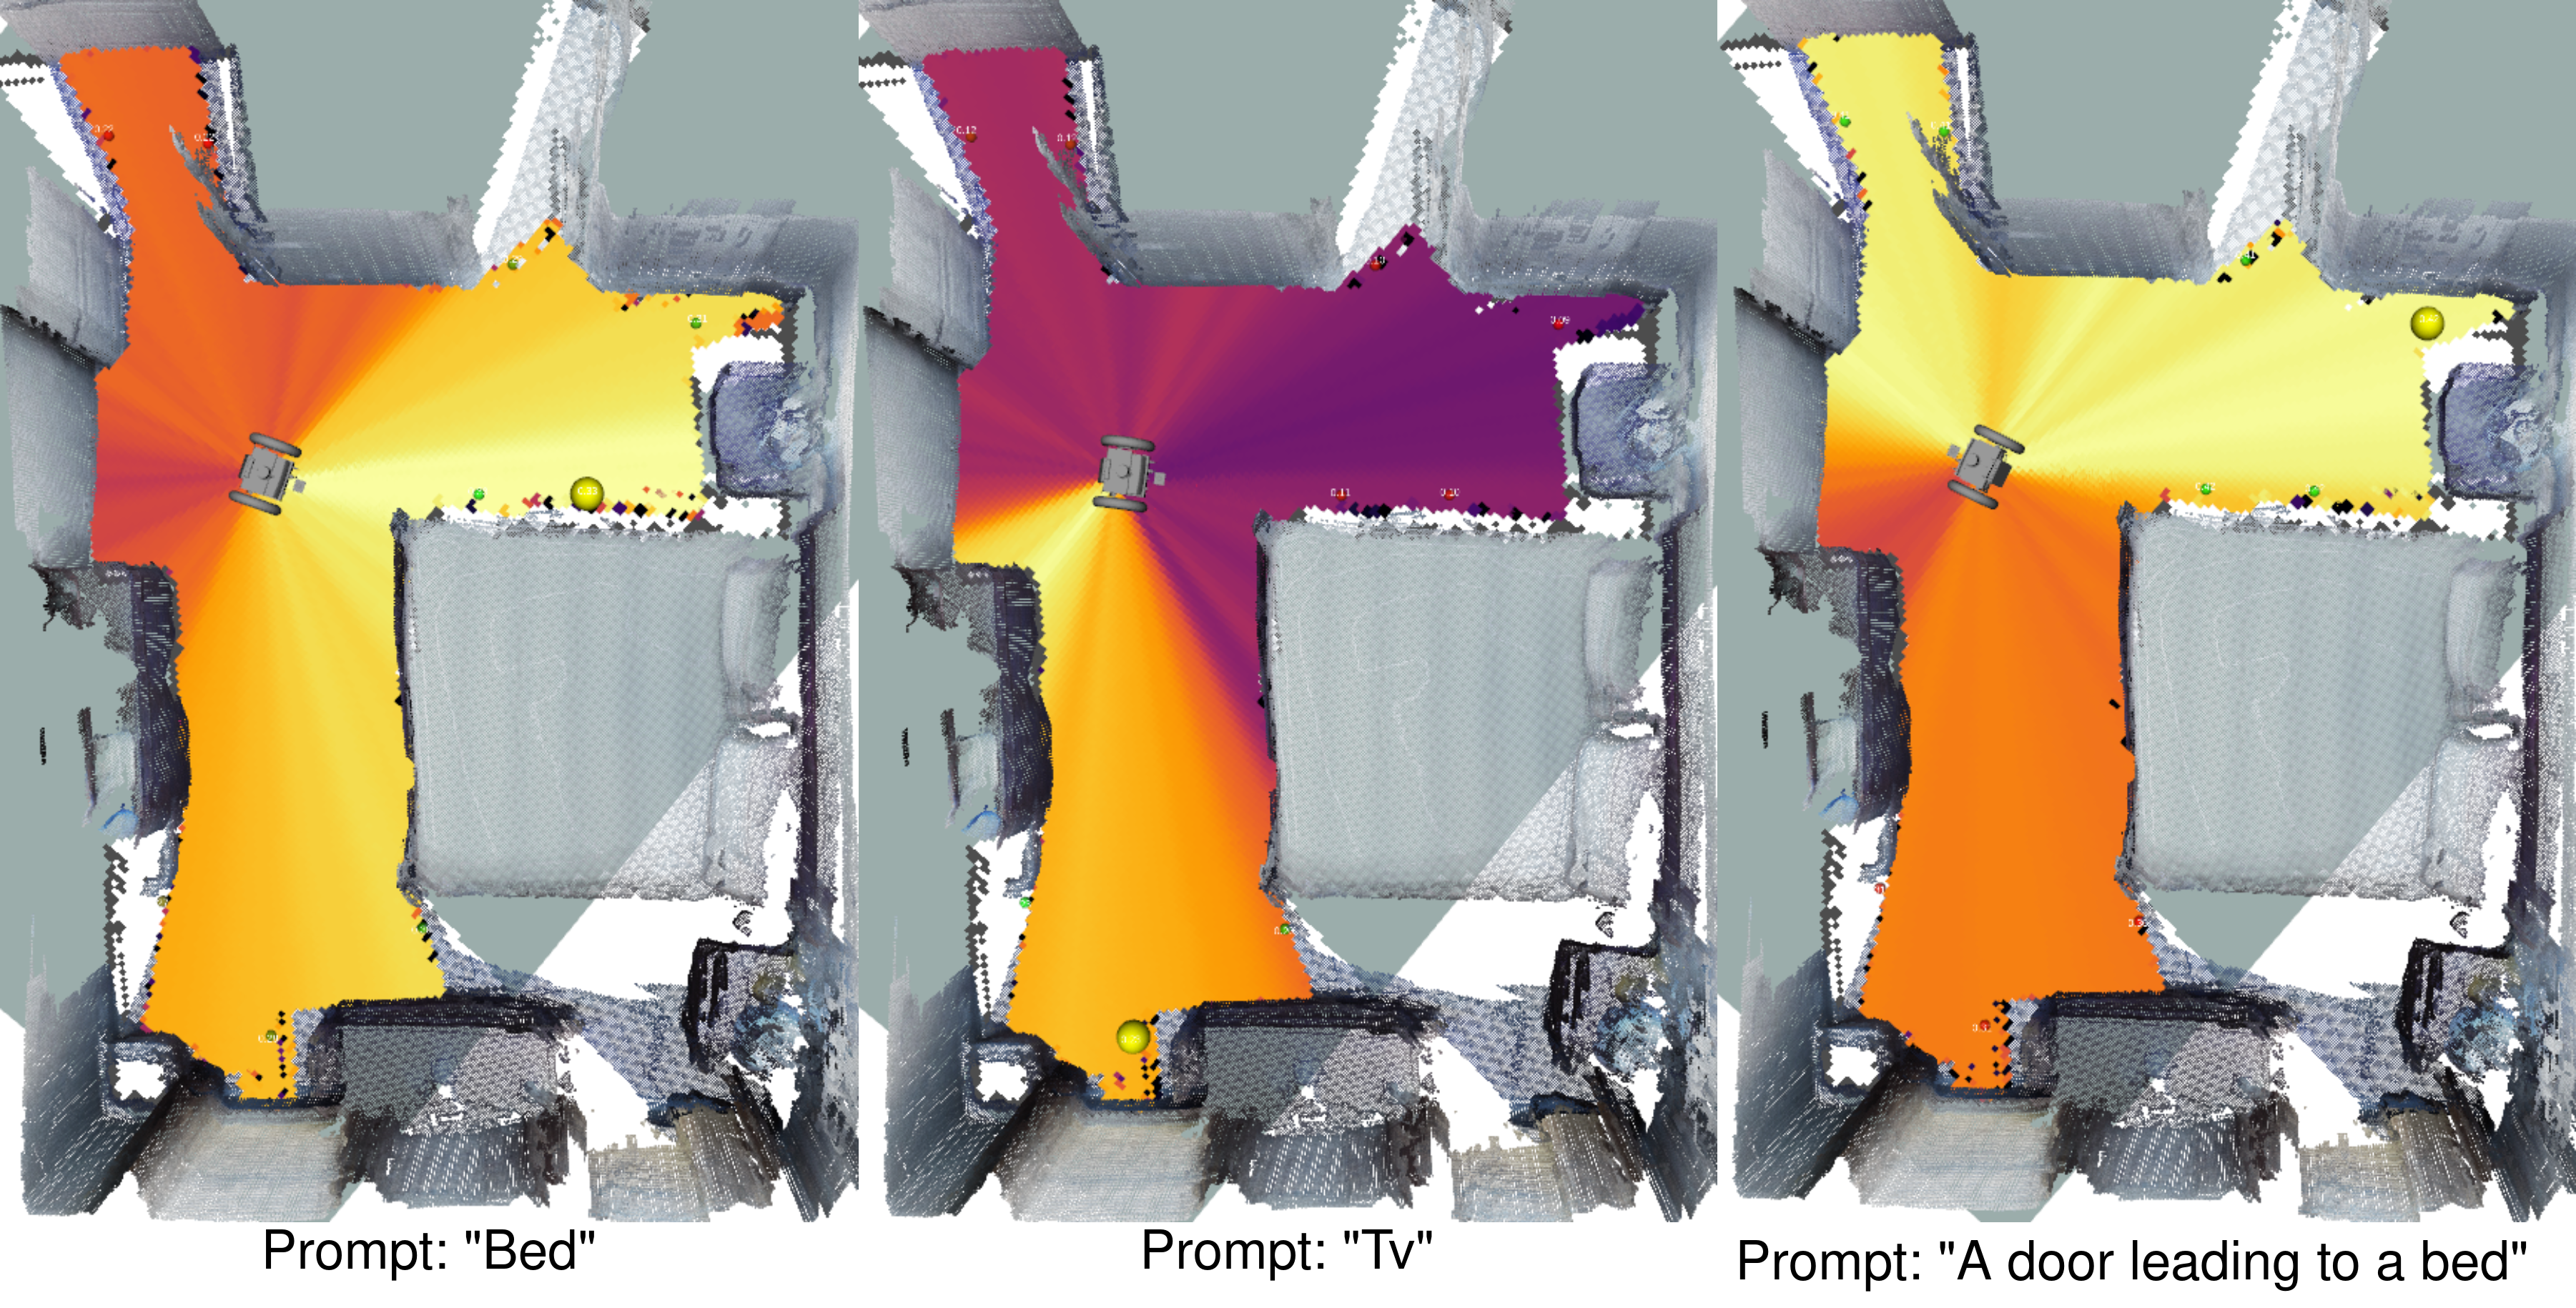
\includegraphics[width=\textwidth]{Images/03_methods/value_map_example.png}
    \caption{Value map example}
    \label{fig:value_map_example}
\end{figure}

\section{Persistent Semantic 3D Mapping} 
\label{sec:methods:persistent_mapping}

\subsection*{Global Map Construction with Open-Fusion}
\begin{itemize}
    \item Incremental creation of a global semantic point cloud map integrating RGB-D observations over time.
    \item Registration of observations using robot poses to maintain a consistent world representation.
    \item Association of semantic labels with 3D points based on query relevance scores.
\end{itemize}

\subsection*{Semantic Clustering and Graph Node Generation}
\begin{itemize}
    \item Clustering of points with similar semantic labels to form object-level hypotheses.
    \item Construction of semantic graph nodes representing detected object instances with aggregated confidence scores.
    \item Maintenance of the semantic graph as a persistent memory for multi-object search tasks.
\end{itemize}

\section{Promptable Zero-Shot Detection} 
\label{sec:methods:zero_shot_detection}
\begin{itemize}
    \item In this work YOLO-E \cite{yoloe} is used as the promptable zero-shot detection model.
    \item YOLO-E has the following advantages:
    \begin{itemize}
        \item High inference speed suitable for real-time applications.
        \item Ability to handle open-vocabulary object detection based on text prompts.
        \item Integration of both visual and textual information for robust detection.
        \item Pre-trained on large-scale datasets, enabling zero-shot generalization to unseen object categories.
    \end{itemize}
\end{itemize}


\subsection*{Open-Vocabulary Object Detection with YOLO-E}
\begin{itemize}
    \item Utilization of the YOLO-E model for open-vocabulary object detection based on text prompts.
    \item Extraction of 2D bounding boxes and associated confidence scores for detected objects.
    \item Segmentation of detected objects to isolate relevant pixels for 3D localization.
\end{itemize}

\subsection*{Depth-Based 3D Localization}
\begin{itemize}
    \item With camera intrinsics and depth information, the 2D bounding boxes ans segmentation masks are projected into 3D space.
    \item Calculation of 3D coordinates for each detected object using depth values within the bounding box.
    \item Semantic detection pointclouds are passed are then clustered and the centroid of each cluster is computed to obtain robust 3D object locations.
    \item For each cluster, the mean of the confidence scores of the associated 2D detections is calculated to assign a confidence score to the 3D localization.
\end{itemize}

\begin{figure}[h!]
    \centering
    \includegraphics[width=1.0\textwidth]{Images/03_methods/vlm_detector.png}
    \caption{YOLO-E detection to graph node 3D localization}
    \label{fig:vlm_detector}
\end{figure}


\section{Fusion Strategy}
\label{sec:methods:fusion_strategy}
\subsection*{Exploration–Memory Weighting}
\begin{itemize}
    \item Exploration and memory graph nodes are fused and weighted as follows:
    \begin{itemize}
        \item Proximity weighting: Nodes closer to the robot's current position are given higher weights, similar to~\cite{bourgaultInformationBasedAdaptive2002}.
        \item Exploration vs Memory: Nodes from the exploration source are prioritized over memory nodes to encourage discovery of new information, similar to~\cite{ramakrishnanPONIPotentialFunctions2022}.
        \item Costmap weighting: Nodes located in areas with lower navigation costs are favored to optimize path planning and navigation efficiency, similar to~\cite{bourgaultInformationBasedAdaptive2002}.
    \end{itemize}
\end{itemize}

\subsection*{Multi-Source Detection Fusion}
\begin{itemize}
    \item Detection graph nodes are weighted based on:
    \begin{itemize}
        \item YOLO-E confidence scores: Higher confidence detections are given more weight.
        \item BLIP-2 value map: Detections with higher semantic relevance to the text prompt are prioritized.
        \item The nearer detection graph nodes are to memory graph nodes, the higher their weight.
    \end{itemize}
\end{itemize}

\subsection*{Relevance Filtering and Node Suppression}
\begin{itemize}
    \item Each source's graph nodes are filtered based on a relevance threshold to eliminate graph nodes within the fov map.
    \item Relevance map is build over time
    \item If a graph node is located in an area that has already been explored and found to be irrelevant to the prompt, it is suppressed.
\end{itemize}

\begin{figure}
    \centering
    \includegraphics[width=1.0\textwidth]{Images/03_methods/3d_relevance_map.png}
    \caption{Fusion strategy for exploration, detection, and memory graph nodes}
    \label{fig:3d_relevance_map}
\end{figure}

\begin{figure}
    \centering
    \includegraphics[width=1.0\textwidth]{Images/03_methods/relevance_map_example.png}
    \caption{Fusion strategy for exploration, detection, and memory graph nodes}
    \label{fig:relevance_map_example}
\end{figure}

\section{Behavior Tree for Semantic-Guided Exploration} 
\label{sec:methods:behavior_tree}

\subsection*{High-Level Task Structure}
\begin{itemize}
    \item The behavior tree (BT) is designed to manage the high-level task structure for semantic-guided exploration.
    \item The BT consists of the following main components:
    \begin{itemize}
        \item Initialization: Clearing Maps, Publishing Prompts
        \item Detection Branch: If object is detected over a threshold, navigate to it, realign to object take picture
        \item Exploration Branch: While object not detected, perform semantic frontier exploration navigating to highest valued frontiers or memory nodes
        \item Termination: If object found, end mission; If time limit reached, end mission
        \item Behavior tree is called with a ros2 action server, which returns on termination success or failure, and actual path taken
    \end{itemize}
\end{itemize}

\begin{figure}[h!]
    \centering
    \includegraphics[width=0.5\textwidth]{Images/03_methods/sage_bt_flowchart.png}
    \caption{System architecture}
    \label{fig:system_overview}
\end{figure}

\subsection*{Integration with Navigation Stack}
\begin{itemize}
    \item Navigation stack used for low-level path planning and obstacle avoidance.
    \item Action used: navigate\_to\_pose, Spin
\end{itemize}
    
\newpage